\begin{surferPage}[Cayley-Cubic]{The Cayley Cubic}
   %This cubic surface (surface of degree $3$) is also contained in the
	Ova kubi\v{c}na ploha (ploha stupnja $3$) se tako\dj{}er nalazi
    %gallery on simple surfaces. 
		u galeriji jednostavnih ploha. 
    %Altogether, it has four double cone singularities.
		Ukupno ima \v{c}etiri singulariteta dvostrukog konusa.
    %It is named after Arthur Cayley who did a lot of research on cubics
		Nazvana je po Arthuru Cayleyu koji je prou\v{c}avao kubike
    %in the $19$th century.
		u 19. stolje\'{c}u.
    
     %However, it was Ludwig Schläfli who first classified these surfaces in 1863 in
		Ludwig Schläfli je 1863. prvi sistemati\v{c}no klasificirao ove plohe 
    %a systematic way with respect to the possible singularities on them.
		s obzirom na njihove mogu\'{c}e singularitete.
    %E.g., in his article one can read why there cannot be more than $4$
		U njegovom \v{c}lanku mo\v{z}ete pro\v{c}itati za\v{s}to kubi\v{c}na ploha
    %singular points on one cubic surface.
		ne mo\v{z}e imati vi\v{s}e od $4$ singularne to\v{c}ke.
    %This yields: $\mu(3)=4$. 
		Vrijedi: $\mu(3)=4$. 
    
    %Around 1900, Felix Klein studied the possible shapes of real cubic surfaces; 
		Oko 1900. Felix Klein se bavio mogu\'{c}im oblicima realnih kubnih ploha;
    %his idea was to answer this question starting from the Cayley Cubic by
		po\v{c}ev\v{s}i od Cayleyeve kubike
    %means of small deformations:
		uz male deformacije:
    %By expanding double cone singularities, disconnecting or merging parts,
		\v{s}ire\'{c}i singularitete dvostrukog konusa, rastavljaju\'{c}i ili spajaju\'{c}i dijelove,
    %he was actually able to find all possible shapes; here are a few of them: 
		uspio je na\'{c}i sve mogu\'{c}e oblike; evo nekih od njih:
    \vspace{0.3cm}
     \begin{center}
      \vspace{-0.2cm}
      \begin{tabular}{@{}c@{\ }c@{\ }c@{\ }c@{}}
        \begin{tabular}{@{}c@{}}
          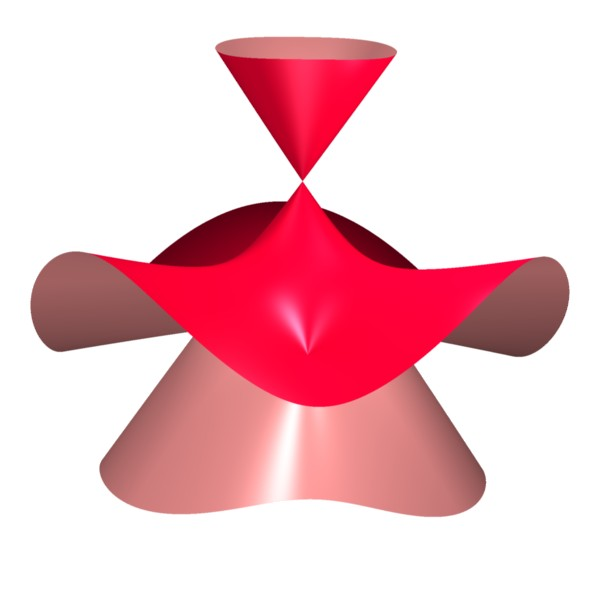
\includegraphics[width=1.35cm]{./../../common/images/cayley_cubic_0}
        \end{tabular}
        &
        \begin{tabular}{@{}c@{}}
          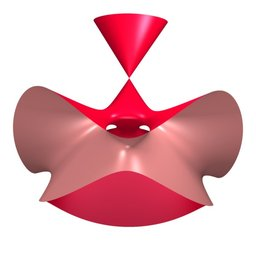
\includegraphics[width=1.35cm]{./../../common/images/cayley_cubic_1}
        \end{tabular}
        &
        \begin{tabular}{@{}c@{}}
          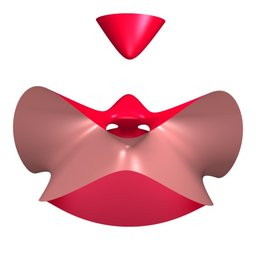
\includegraphics[width=1.35cm]{./../../common/images/cayley_cubic_2}
        \end{tabular}
        &
        \begin{tabular}{@{}c@{}}
          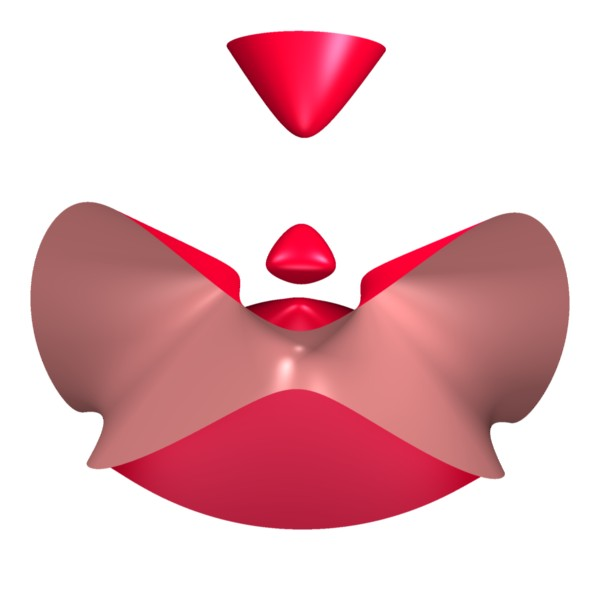
\includegraphics[width=1.35cm]{./../../common/images/cayley_cubic_3}
        \end{tabular}
      \end{tabular}
    \end{center}
\end{surferPage}
